\chapter{الدورية}\label{ch:b1:periodicity}

الليثيوم والصوديوم والبوتاسيوم فلزات طرية لامعة يبهت سطحها في الهواء
وتتفاعل مع الماء؛ والفلور والكلور والبروم لافلزات ملوّنة أكّالة تنتزع
الإلكترونات من كل شيء تقريبًا. وكل ثلاثي منها يقع في عمود واحد من الجدول
الدوري، وأعضاء العمود الواحد يتشابهون، في حين لا يتشابه الجيران على
امتداد السطر. وقد فسّر الفصل السابق السبب: لعناصر العمود الواحد توزيع
\omterm{def:b1:quantum-numbers:configuration}{إلكترونات التكافؤ} نفسه. ويحوّل هذا الفصل ذلك التفسير إلى أعداد ---
أنصاف أقطار، وطاقات تأين، وألفات إلكترونية، وكهرسلبيات --- وإلى منحيات
تتيح للكيميائي أن يتنبأ، من موضع العنصر وحده، بحجم ذراته، وبمدى سهولة
تخليها عن الإلكترونات أو تقبّلها لها، وبالجهة التي تميل إليها إلكترونات
الرابطة.

\begin{recall}
تبدأ كل \omterm{def:b1:periodicity:table}{دورة} بملء \omterm{def:b1:quantum-numbers:orbital}{طبقة فرعية} \babelsublr{$n$s} وتنتهي \omterm{def:b1:quantum-numbers:orbital}{بطبقة فرعية} \babelsublr{$n$p} ممتلئة؛ وعروض
الفئات s وp وd وf هي 2 و6 و10
و14 (\cref{prop:b1:quantum-numbers:table}). ووصف الكتاب الأول (الصف
الحادي عشر) \omterm{def:b1:periodicity:electronegativity}{الكهرسلبية} بأنها نزعة الذرة إلى جذب
إلكترونات الرابطة.
\end{recall}

\section{الجدول مبنيًّا من التوزيعات}

\begin{definition}[الدورة، الزمرة، الفئة]\label{def:b1:periodicity:table}
تُرتَّب العناصر في الجدول الدوري بحسب تزايد عددها
الذري $Z$. \emph{الدورة}\index{دورة} سطر: هي العناصر التي لطبقة
تكافئها العدد الرئيسي $n$ نفسه. و\emph{الزمرة}\index{زمرة} عمود،
مرقّم من 1 إلى 18: هي العناصر التي لها توزيع التكافؤ نفسه.
و\emph{الفئة}\index{فئة} مجموعة العناصر التي آخر \omterm{def:b1:quantum-numbers:orbital}{طبقة فرعية} تمتلئ فيها
من نوع واحد، s أو p أو d أو f.
\end{definition}

\begin{example}[قراءة موضع]\label{ex:b1:periodicity:position}
السيلينيوم، $[\ce{Ar}]\,3\text{d}^{10} 4\text{s}^2 4\text{p}^4$، في
\omterm{def:b1:periodicity:table}{الدورة} 4 (طبقة التكافؤ $n = 4$)، وفي \omterm{def:b1:periodicity:table}{الفئة} p، وفي \omterm{def:b1:periodicity:table}{الزمرة} 16 (إلكترونا s،
وعشرة إلكترونات d، وأربعة p: $2 + 10 + 4$)؛ وتوزيع تكافئه
$n\text{s}^2 n\text{p}^4$ هو توزيع الأكسجين والكبريت الواقعين فوقه.
\end{example}

\begin{definition}[الفلز، اللافلز، شبه الفلز]\label{def:b1:periodicity:metalloid}
الفلز عنصر يوصل جسمه الصلب الكهرباء وتفقد ذراته الإلكترونات بسهولة
فتكوّن كاتيونات؛ واللافلز عنصر لا يوصل (مع استثناءات مثل الغرافيت)
ويكتسب الإلكترونات أو يشارك بها بسهولة. و\emph{شبه الفلز}\index{شبه فلز}
عنصر ذو طابع وسيط، شبه موصل: البور، والسيليكون،
والجرمانيوم، والزرنيخ، والأنتيمون، والتيلوريوم.
\end{definition}

\begin{omfigure}
\omperiodictable[colour=metals, legend, f block=false]

{\small الفلزات (وهي الغالبية العظمى)، وأشباه الفلزات على امتداد درج من
البور إلى التيلوريوم، واللافلزات في الأعلى يمينًا. أما \omterm{def:b1:periodicity:table}{الفئة} f،
المحذوفة هنا، فكلها فلزات.}
\end{omfigure}

\section{الحجم: أنصاف الأقطار الذرية والأيونية}

\begin{definition}[الحجب، الشحنة النووية الفعلية]\label{def:b1:periodicity:screening}
في ذرة ذات عدة إلكترونات، يُجذب الإلكترون بالنواة، التي شحنتها $Ze$،
ويُدفع بالإلكترونات الأخرى. وتلغي \omterm{def:b1:quantum-numbers:configuration}{الإلكترونات الداخلية} جزءًا من جذب
النواة: هذا هو \emph{الحجب}\index{حجب}. فيسلك \omterm{def:b1:quantum-numbers:configuration}{إلكترون التكافؤ} كأنه
يحس بشحنة نووية مخفَّضة $Z^{*}e$، هي \emph{الشحنة النووية
الفعلية}\index{شحنة نووية فعلية}، مع $Z^{*} < Z$. وإلكترونات
الطبقة الداخلية تحجب حجبًا شبه تام؛ أما إلكترونات الطبقة نفسها
فلا تحجب إلا قليلًا.
\end{definition}

\begin{remark}[أداة نوعية]\label{rem:b1:periodicity:slater}
يُستعمل $Z^{*}$ في هذا الكتاب استعمالًا نوعيًا: على امتداد \omterm{def:b1:periodicity:table}{الدورة}، يزداد
$Z$ بواحد في كل خطوة، في حين لا يحجب الإلكترون المضاف، وهو في الطبقة
نفسها، إلا قليلًا، فيزداد $Z^{*}$ الذي تحس به \omterm{def:b1:quantum-numbers:configuration}{إلكترونات التكافؤ}؛ ونزولًا
في \omterm{def:b1:periodicity:table}{الزمرة}، يتغير $Z^{*}$ قليلًا لكن طبقة التكافؤ
$n$ تكبر. أما قواعد حساب $Z^{*}$ من التوزيع (قواعد سلاتر) فيعطيها
مجلد السنة الثانية.
\end{remark}

\begin{definition}[نصف القطر التساهمي، نصف القطر الأيوني]\label{def:b1:periodicity:radius}
\emph{نصف القطر التساهمي}\index{نصف قطر تساهمي} لعنصر هو نصف
طول رابطة أحادية بين ذرتين منه: ففي الكلور هو نصف
المسافة \ce{Cl-Cl} في \ce{Cl2}. و\emph{نصف القطر
الأيوني}\index{نصف قطر أيوني} لأيون هو حصته من المسافة بين الكاتيونات
والأنيونات المتجاورة في البلورات الأيونية، وفق اصطلاح يثبّت نصف قطر
أيون مرجعي واحد
(\ce{O^{2-}})؛ وهو يتعلق قليلًا بعدد الجيران.
\end{definition}

\begin{example}[الهالوجينات]\label{ex:b1:periodicity:halogen-radii}
أطوال روابط \ce{F2} و\ce{Cl2} و\ce{Br2} و\ce{I2} هي 141.2
و198.8 و228.1 و\qty{266.6}{pm}، فأنصاف الأقطار التساهمية 71 و99 و114
و\qty{133}{pm}: كل خطوة نزولًا في \omterm{def:b1:periodicity:table}{الزمرة} تضيف طبقة ونحو
\qty{20}{pm} أو أكثر.
% ledger: re:F2, re:Cl2, re:Br2, re:I2
\end{example}

\begin{proposition}[منحى نصف القطر]\label{prop:b1:periodicity:radius-trend}
تتناقص أنصاف الأقطار الذرية من اليسار إلى اليمين على امتداد \omterm{def:b1:periodicity:table}{الدورة}،
وتتزايد من الأعلى إلى الأسفل نزولًا في \omterm{def:b1:periodicity:table}{الزمرة}. والكاتيون أصغر من ذرته،
والأنيون أكبر؛ وفي سلسلة متساوية الإلكترونات (أيونات لها التوزيع
نفسه) يتناقص نصف القطر كلما ازداد $Z$.
\end{proposition}

\begin{proof}[استدلال]
حجم الذرة هو حجم مداراتها التكافؤية، التي تنكمش
حين يكبر $Z^{*}$ وتنتفخ حين يكبر $n$. وعلى امتداد \omterm{def:b1:periodicity:table}{الدورة} يكون $n$ ثابتًا
و$Z^{*}$ متزايدًا: فتنكمش الذرات. ونزولًا في \omterm{def:b1:periodicity:table}{الزمرة} يكبر $n$ بواحد في
كل خطوة، وهذا يرجح على التغير الصغير في $Z^{*}$. والكاتيون قد فقد
طبقة تكافئه، أو إلكترونات كان يدفع بعضها بعضًا؛ والأنيون قد
اكتسب إلكترونًا يدفع الإلكترونات الأخرى. وفي السلسلة المتساوية الإلكترونات
تمسك نواةٌ متزايدة الشحنة الإلكتروناتِ نفسها.
\end{proof}

\begin{omfigure}
\begin{tikzpicture}[font=\small, x=1pt, y=1pt]
  % ledger: rion:O2-VI, rion:F-VI, rion:Na+VI, rion:Mg2+VI, rion:Al3+VI
  % radii in pm drawn at 0.30 pt per pm (circles to scale)
  \foreach \x/\r/\lab/\v in {40/140/\ce{O^{2-}}/140, 130/133/\ce{F-}/133,
      210/102/\ce{Na+}/102, 275/72/\ce{Mg^{2+}}/72, 325/53.5/\ce{Al^{3+}}/54} {
    \draw[fill=omDef!20, draw=omDef!70!black] (\x,0) circle ({0.30*\r});
    \node at (\x,0) {\lab};
    \node[below] at (\x,-50) {\v\,pm};
  }
  \node[anchor=west, align=left] at (350,0) {\foreignlanguage{arabic}{عشرة إلكترونات لكل منها،}\\$Z = 8 \to 13$};
\end{tikzpicture}

{\small السلسلة المتساوية الإلكترونات $1\text{s}^2 2\text{s}^2 2\text{p}^6$،
مرسومة بمقياس صحيح (أنصاف أقطار أيونية لستة جيران). الإلكترونات العشرة
نفسها تنكمش كلما كبرت الشحنة النووية.}
\end{omfigure}

\section{الطاقات: التأين والألفة الإلكترونية}

\begin{definition}[طاقات التأين]\label{def:b1:periodicity:ionisation-energy}
\emph{طاقة التأين الأولى}\index{طاقة التأين الأولى} $E_{i1}$
لعنصر هي الطاقة اللازمة لنزع إلكترون واحد من
الذرة المعزولة في حالتها الأساسية، في الطور الغازي:
\[
  \ce{X(g) -> X+(g) + e-}, \qquad E_{i1} = E(\ce{X+}) + E(\ce{e-}) - E(\ce{X}) > 0 .
\]
و\emph{طاقات التأين المتتالية}\index{طاقات التأين المتتالية}
$E_{i2}, E_{i3}, \dots$ تنزع الإلكترون الثاني، فالثالث\dots\ من
\ce{X+}، ثم \ce{X^{2+}}\dots\ وتُعطى بالإلكترون فولت لكل ذرة
أو بالكيلوجول لكل مول
($\qty{1}{eV} \leftrightarrow \qty{96.49}{kJ/mol}$).
% ledger: const:NA, const:e (1 eV x N_A = 96.485 kJ/mol)
\end{definition}

\begin{omfigure}
\begin{tikzpicture}
\begin{axis}[
  width=0.92\linewidth, height=6.4cm,
  xmin=0, xmax=37, ymin=0, ymax=27,
  axis x line=bottom, axis y line=left,
  xlabel={\foreignlanguage{arabic}{العدد الذري $Z$}}, ylabel={\babelsublr{$E_{i1}$ (eV)}},
  xtick={2,10,18,36}, ytick={0,5,10,15,20,25},
  tick label style={font=\small}, label style={font=\small},
  clip=false]
\addplot[omDef, thick, mark=*, mark size=1.3pt] table[x=Z, y=IE_eV] {figdata/out/bachelor-1-ionisation-energies.dat};
\node[font=\small, anchor=south] at (axis cs:2,24.6) {He};
\node[font=\small, anchor=south] at (axis cs:10,21.6) {Ne};
\node[font=\small, anchor=south] at (axis cs:18,15.8) {Ar};
\node[font=\small, anchor=south] at (axis cs:36,14.0) {Kr};
\node[font=\small, anchor=north] at (axis cs:3,5.2) {Li};
\node[font=\small, anchor=north] at (axis cs:11,4.9) {Na};
\node[font=\small, anchor=north] at (axis cs:19,4.1) {K};
\node[font=\small, anchor=north] at (axis cs:31,5.8) {Ga};
\node[font=\small, anchor=north] at (axis cs:5,7.9) {B};
\node[font=\small, anchor=north] at (axis cs:8,13.2) {O};
\node[font=\small, anchor=north west] at (axis cs:13.1,6.0) {Al};
\node[font=\small, anchor=north] at (axis cs:16,9.9) {S};
\node[font=\small, anchor=south] at (axis cs:26,8.0) {\foreignlanguage{arabic}{فلزات \babelsublr{3d}}};
\end{axis}
\end{tikzpicture}

{\small طاقات التأين الأولى للعناصر الستة والثلاثين الأولى. قيمها العظمى عند
الغازات النبيلة، والصغرى عند الفلزات القلوية؛ والانخفاضات الصغيرة عند B وAl وGa
وعند O وS هي آثار الطبقات الفرعية في
\cref{prop:b1:periodicity:ie-anomalies}.}
\end{omfigure}

\begin{proposition}[منحى طاقة التأين]\label{prop:b1:periodicity:ie-trend}
تتزايد \omterm{def:b1:periodicity:ionisation-energy}{طاقة التأين الأولى} على امتداد \omterm{def:b1:periodicity:table}{الدورة}، من الفلز
القلوي إلى الغاز النبيل، وتتناقص نزولًا في \omterm{def:b1:periodicity:table}{الزمرة}. \omterm{def:b1:periodicity:ionisation-energy}{وطاقات التأين
المتتالية} متزايدة دائمًا، $E_{i1} < E_{i2} < \dots$، وتقفز
بعامل كبير حين ينتمي الإلكترون المنزوع إلى طبقة داخلية.
\end{proposition}

\begin{proof}[استدلال]
يكون نزع الإلكترون أسهل حين يكون بعيدًا عن النواة ويحس
بقيمة صغيرة للمقدار $Z^{*}$: على امتداد \omterm{def:b1:periodicity:table}{الدورة} يكبر $Z^{*}$ ويصغر نصف القطر؛
ونزولًا في \omterm{def:b1:periodicity:table}{الزمرة} يكبر نصف القطر. وكل إلكترون تالٍ يُنتزع من أيون
أعلى شحنةً وأصغر حجمًا، فيكلّف أكثر؛ ومتى فرغت طبقة التكافؤ
جاء الإلكترون التالي من طبقة ذات $n$ أصغر، أقرب كثيرًا
إلى النواة وتكاد لا تُحجب أبدًا.
\end{proof}

\begin{example}[المغنيسيوم]\label{ex:b1:periodicity:magnesium}
\omterm{def:b1:periodicity:ionisation-energy}{طاقات التأين المتتالية} للمغنيسيوم هي 7.65 و15.04 و80.14
و\qty{109.27}{eV}. فالنسبة $E_{i2}/E_{i1} \approx 2$ معتدلة؛
أما $E_{i3}/E_{i2} \approx 5.3$ فقفزة: الإلكترون الثالث يأتي من
قلب 2p. فيتخلى المغنيسيوم عن إلكترونيه 3s ويقف عند
\ce{Mg^{2+}}، ذي توزيع الغاز النبيل النيون.
% ledger: ie:Mg, ie2:Mg, ie3:Mg, ie4:Mg
\end{example}

\begin{omfigure}
\begin{tikzpicture}
\begin{axis}[
  width=0.55\linewidth, height=5.2cm, ybar, bar width=14pt,
  xmin=0.4, xmax=4.6, ymin=1, ymax=300, ymode=log,
  axis x line=bottom, axis y line=left,
  xlabel={الإلكترون المنزوع}, ylabel={\babelsublr{$E_{i}$ (eV)}},
  xtick={1,2,3,4}, xticklabels={{الأول},{الثاني},{الثالث},{الرابع}},
  tick label style={font=\small}, label style={font=\small},
  nodes near coords={\pgfmathprintnumber[fixed, fixed zerofill, precision=2]{\pgfplotspointmeta}},
  nodes near coords style={font=\scriptsize},
  point meta=rawy]
\addplot[fill=omDef!40, draw=omDef] table[x=k, y=IE_eV] {figdata/out/bachelor-1-ionisation-energies-mg.dat};
\end{axis}
\end{tikzpicture}

{\small \omterm{def:b1:periodicity:ionisation-energy}{طاقات التأين المتتالية} للمغنيسيوم (محور لوغاريتمي).
الثالثة خمسة أضعاف الثانية: فقد فرغت الطبقة 3s وبُلغ
القلب.}
\end{omfigure}

\begin{proposition}[انخفاضان على امتداد الدورة]\label{prop:b1:periodicity:ie-anomalies}
على امتداد الدورتين 2 و3، تنخفض \omterm{def:b1:periodicity:ionisation-energy}{طاقة التأين الأولى} قليلًا من
\omterm{def:b1:periodicity:table}{الزمرة} 2 إلى \omterm{def:b1:periodicity:table}{الزمرة} 13 (من \ce{Be} إلى \ce{B}، ومن \ce{Mg} إلى \ce{Al}) ومن
\omterm{def:b1:periodicity:table}{الزمرة} 15 إلى \omterm{def:b1:periodicity:table}{الزمرة} 16 (من \ce{N} إلى \ce{O}، ومن \ce{P} إلى \ce{S}).
\end{proposition}

\begin{proof}[استدلال]
في \ce{B} و\ce{Al} يكون الإلكترون المنزوع أول إلكترون p،
وهو أعلى طاقةً من إلكترونات s في \ce{Be} و\ce{Mg}. وفي \ce{O}
و\ce{S} يكون الإلكترون المنزوع رابع إلكترون p، وهو أول من
يشارك غيره مدارًا (\omorbs{ud,u,u}): فتنافره مع شريكه يجعل
نزعه أسهل من نزع إلكترون من \omterm{def:b1:quantum-numbers:orbital}{الطبقة الفرعية} نصف الممتلئة في
\ce{N} أو \ce{P} (\omorbs{u,u,u}).
% ledger: ie:Be, ie:B, ie:N, ie:O, ie:Mg, ie:Al, ie:P, ie:S
\end{proof}

\begin{definition}[الألفة الإلكترونية]\label{def:b1:periodicity:electron-affinity}
\emph{الألفة الإلكترونية}\index{ألفة إلكترونية} $E_{ea}$
لعنصر هي الطاقة المحرَّرة حين تأسر ذرة معزولة في حالتها الأساسية
إلكترونًا في الطور الغازي،
\[
  \ce{X(g) + e- -> X-(g)}, \qquad E_{ea} = E(\ce{X}) + E(\ce{e-}) - E(\ce{X-}) .
\]
وتكون موجبة حين يكون الأنيون أكثر استقرارًا من الذرة والإلكترون
الحر.
\end{definition}

\begin{example}[الهالوجينات وجيرانها]\label{ex:b1:periodicity:ea}
الألفات الإلكترونية للعناصر \ce{F} و\ce{Cl} و\ce{Br} و\ce{I} هي 3.40
و3.61 و3.36 و\qty{3.06}{eV}، وهي الأكبر بين كل العناصر؛ وألفتا
\ce{O} و\ce{S} هما 1.44 و\qty{2.02}{eV}، وألفة \ce{C} \qty{1.26}{eV}،
وألفة \ce{Na} \qty{0.55}{eV}. فالذرات التي تكمل \omterm{def:b1:quantum-numbers:orbital}{طبقة فرعية} بأسرها
إلكترونًا (الهالوجينات) تحرر طاقة كبيرة. أما النيتروجين والبيريليوم
والمغنيسيوم والغازات النبيلة فلا تكوّن أنيونًا غازيًا مستقرًا: إذ يتعين على
الإلكترون الزائد أن يقترن في \omterm{def:b1:quantum-numbers:orbital}{طبقة فرعية} p نصف ممتلئة أو أن يدخل \omterm{def:b1:quantum-numbers:orbital}{طبقة فرعية}
جديدة. وألفة الفلور أصغر من ألفة الكلور لأن الإلكترون المضاف يُحشر
في الطبقة 2p الصغيرة.
% ledger: ea:F, ea:Cl, ea:Br, ea:I, ea:O, ea:S, ea:C, ea:Na
\end{example}

\section{الكهرسلبية وقابلية الاستقطاب}

\begin{definition}[الكهرسلبية]\label{def:b1:periodicity:electronegativity}
\emph{الكهرسلبية}\index{كهرسلبية} $\chi$ لعنصر تقيس
نزعة ذراته، في جزيء، إلى جذب
إلكترونات الروابط التي تكوّنها. وهناك سلّمان مستعملان.
\begin{itemize}
  \item في \emph{سلّم بولينغ}\index{سلم بولينغ}، تُعرَّف الفروق
        انطلاقًا من طاقات الروابط $D$:
        \[
          |\chi_A - \chi_B| = \sqrt{\frac{\Delta E}{\qty{1}{eV}}}, \qquad
          \Delta E = D(\text{A--B}) - \tfrac12\big[D(\text{A--A}) +
          D(\text{B--B})\big],
        \]
        ويُثبَّت السلّم بالقيمة $\chi(\ce{F}) = 3.98$.
  \item في \emph{سلّم موليكن}\index{سلم موليكن}،
        $\chi_M = \tfrac12\,(E_{i1} + E_{ea})$، بالإلكترون فولت.
\end{itemize}
\end{definition}

\begin{remark}[لماذا طاقة الرابطة الزائدة]\label{rem:b1:periodicity:pauling}
لو جذبت ذرتا الرابطة A--B إلكتروناتها بالتساوي لكانت طاقة الرابطة
قريبة من متوسط طاقتي A--A وB--B. فإذا كانت إحدى الذرتين أكثر كهرسلبية
اكتسبت الرابطة طابعًا أيونيًا
جزئيًا، $\ce{A^{\delta+}-B^{\delta-}}$، يضيف تجاذبه الكهربائي الساكن
طاقةً: فالمقدار $\Delta E > 0$ يقيس عدم تكافؤ المشاركة. ويقول تعريف
موليكن الشيء نفسه من جهة الذرات: فالذرة التي تمسك إلكتروناتها
بقوة ($E_i$ كبيرة) وترحّب بإلكترون زائد
($E_{ea}$ كبيرة) تجذب إلكترونات الرابطة.
\end{remark}

\begin{omfigure}
% ledger: en:H, en:Li, en:Be, en:B, en:C, en:N, en:O, en:F, en:Na, en:Mg,
% en:Al, en:Si, en:P, en:S, en:Cl, en:K, en:Ca, en:Ga, en:Ge, en:As, en:Se,
% en:Br, en:Rb, en:Sr, en:In, en:Sn, en:Sb, en:Te, en:I, en:Cs, en:Ba
\omperiodictable[upto=56, f block=false, numbers=false, highlight colour=omDef!12,
  highlight={F,O,N,Cl}, values={H/2.20,Li/0.98,Be/1.57,B/2.04,C/2.55,N/3.04,O/3.44,F/3.98,
  Na/0.93,Mg/1.31,Al/1.61,Si/1.90,P/2.19,S/2.58,Cl/3.16,K/0.82,Ca/1.00,Ga/1.81,Ge/2.01,
  As/2.18,Se/2.55,Br/2.96,Rb/0.82,Sr/0.95,In/1.78,Sn/1.96,Sb/2.05,Te/2.10,I/2.66,
  Cs/0.79,Ba/0.89}]

{\small كهرسلبيات بولينغ لعناصر الزمر الرئيسية (تُركت \omterm{def:b1:periodicity:table}{الفئة} d
فارغة). تتزايد من اليسار إلى اليمين ومن الأسفل إلى
الأعلى؛ والعناصر الأربعة الأكثر كهرسلبية، F وO وCl وN، مظللة.}
\end{omfigure}

\begin{proposition}[منحى الكهرسلبية]\label{prop:b1:periodicity:en-trend}
تتزايد \omterm{def:b1:periodicity:electronegativity}{الكهرسلبية} على امتداد \omterm{def:b1:periodicity:table}{الدورة} وتتناقص نزولًا في \omterm{def:b1:periodicity:table}{الزمرة}:
فالفلور أكثر العناصر كهرسلبية، والسيزيوم والفرانسيوم
أقلها. ويعطي الفرق $\Delta\chi$ بين ذرتين مترابطتين
طابع الرابطة: $\Delta\chi < 0.4$ تساهمية شبه غير قطبية،
و$0.4 < \Delta\chi < 1.7$ تساهمية قطبية، و$\Delta\chi > 1.7$ أيونية أساسًا
--- ثلاث مناطق من متصل، لا أصناف حادة الحدود.
\end{proposition}

\begin{example}[ثلاث روابط]\label{ex:b1:periodicity:bonds}
\ce{C-H}: $\Delta\chi = 2.55 - 2.20 = 0.35$، شبه غير قطبية؛
\ce{O-H}: $3.44 - 2.20 = 1.24$، قطبية، والأكسجين يحمل شحنة جزئية
سالبة؛ \ce{Na-Cl}: $3.16 - 0.93 = 2.23$، أيونية.
% ledger: en:C, en:H, en:O, en:Na, en:Cl
\end{example}

\begin{definition}[قابلية الاستقطاب]\label{def:b1:periodicity:polarisability}
\emph{قابلية الاستقطاب}\index{قابلية الاستقطاب} لذرة أو أيون أو
جزيء تقيس مدى سهولة تشوّه سحابته الإلكترونية تحت تأثير
مجال كهربائي --- مجال أيون أو ثنائي قطب مجاور. فالنوع
القابل للاستقطاب يكتسب، في مجال، عزم ثنائي قطب محرَّضًا
متناسبًا مع المجال.
\end{definition}

\begin{proposition}[منحى قابلية الاستقطاب]\label{prop:b1:periodicity:polarisability-trend}
تكبر \omterm{def:b1:periodicity:polarisability}{قابلية الاستقطاب} مع حجم السحابة الإلكترونية ومع
عدد الإلكترونات، وتصغر مع شحنة النواة التي
تمسكها: فهي تتزايد نزولًا في \omterm{def:b1:periodicity:table}{الزمرة} ($\ce{F-} < \ce{Cl-} < \ce{Br-} <
\ce{I-}$)، والأنيونات أكثر قابلية للاستقطاب بكثير من الكاتيونات، والأنيونات
الكبيرة الرخوة مثل \ce{I-} أكثر الأنواع الشائعة قابلية للاستقطاب.
\end{proposition}

\begin{example}[لماذا تهم قابلية الاستقطاب]\label{ex:b1:periodicity:pol}
يكبر تجاذب لندن بين الجزيئات، وهو موضوع
\cref{ch:b1:intermolecular-forces-solvents}، مع \omterm{def:b1:periodicity:polarisability}{قابلية الاستقطاب}:
فثنائي اليود جسم صلب في درجة حرارة الغرفة، وثنائي الكلور غاز. وفي البلورة
الأيونية، يستقطب كاتيون صغير عالي الشحنة أنيونًا كبيرًا فيمنح
الرابطة شيئًا من الطابع التساهمي، وهو قصور النموذج الأيوني البسيط
الذي نلقاه في \cref{ch:b1:crystals-ionic-covalent}.
\end{example}

\begin{history}[سلّم بولينغ، 1932]
لاحظ الكيميائي الأمريكي لينوس بولينغ سنة 1932 أن طاقة الرابطة
بين ذرتين مختلفتين تكاد تكون دائمًا أكبر من متوسط طاقتي الرابطتين
المتناظرتين، فبنى من هذا الفائض أول سلّم \omterm{def:b1:periodicity:electronegativity}{للكهرسلبية}. ولا يزال سلّمه،
بعد مراجعته كلما قيست طاقات روابط أدق، هو الوارد في كل جدول.
ونال بولينغ جائزة نوبل في الكيمياء سنة 1954 لأعماله في
الرابطة الكيميائية، ثم جائزة نوبل للسلام سنة 1962.
\end{history}

\begin{omfigure}
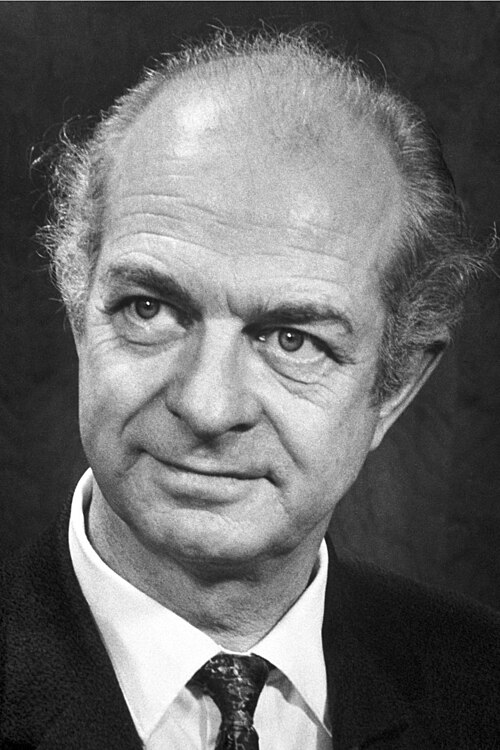
\includegraphics[width=0.24\linewidth]{images/book2/pauling.jpg}

{\small لينوس بولينغ (1901--1994).}
\end{omfigure}

\section{منحيات الطابع الكيميائي}

\begin{proposition}[الطابع المختزل والطابع المؤكسد]\label{prop:b1:periodicity:redox-trend}
العناصر ذات طاقة التأين المنخفضة \omterm{def:b1:periodicity:electronegativity}{والكهرسلبية} المنخفضة، في يسار
الجدول وفي أسفل زمرها، تفقد الإلكترونات بسهولة:
فهي فلزات مختزلة (والفلزات القلوية أكثرها). والعناصر ذات
\omterm{def:b1:periodicity:electronegativity}{الكهرسلبية} \omterm{def:b1:periodicity:electron-affinity}{والألفة الإلكترونية} العاليتين، في الأعلى يمينًا، تكتسب
الإلكترونات بسهولة: فهي لافلزات مؤكسدة (والفلور والأكسجين
والكلور أكثرها). أما الغازات النبيلة، بطاقة تأينها العالية وانعدام
ألفتها لإلكترون زائد، فلا تفعل هذا ولا ذاك.
\end{proposition}

\begin{method}[التنبؤ بمنحى من الموضع]\label{met:b1:periodicity:predict}
لمقارنة عنصرين في خاصية مرتبطة بقبضة النواة
على \omterm{def:b1:quantum-numbers:configuration}{إلكترونات التكافؤ} (نصف القطر، $E_i$، $E_{ea}$، $\chi$):
\begin{enumerate}
  \item إن كانا في \omterm{def:b1:periodicity:table}{الزمرة} نفسها، فالأدنى منهما له العدد $n$
        الأكبر: نصف قطر أكبر، و$E_i$ و$\chi$ أصغر؛
  \item إن كانا في \omterm{def:b1:periodicity:table}{الدورة} نفسها، فالأبعد يمينًا له
        $Z^{*}$ الأكبر: نصف قطر أصغر، و$E_i$ و$\chi$ أكبر؛
  \item وإلا فقارن كلًّا منهما بالعنصر الواقع عند تقاطع
        سطره وعمود الآخر؛
  \item تحقق من آثار الطبقات الفرعية (بداية \omterm{def:b1:quantum-numbers:orbital}{طبقة فرعية} p، أول إلكترون p
        مقترن) قبل الاستنتاج بشأن طاقات التأين.
\end{enumerate}
\end{method}

\begin{example}[الليثيوم في البطارية]\label{ex:b1:periodicity:lithium}
لليثيوم أدنى \omterm{def:b1:periodicity:electronegativity}{كهرسلبية} في \omterm{def:b1:periodicity:table}{الدورة} 2، ويفقد إلكترونه 2s
بسهولة، وهو في الوقت نفسه أخف الفلزات: فهو يحمل أكبر شحنة قابلة
للنقل لكل غرام بين كل العناصر، ولهذا يغذي البطاريات
القابلة لإعادة الشحن. وطاقة تأينه الأولى، \qty{5.39}{eV}، أكبر
من طاقة تأين الصوديوم (5.14) أو البوتاسيوم (4.34)، ومع ذلك فهو في الماء
أشد الفلزات القلوية اختزالًا، وهي مفارقة يحلها شدة
إماهة الأيون الصغير \ce{Li+} (\cref{ch:b1:nernst}).
% ledger: ie:Li, ie:Na, ie:K
\end{example}

\section{تمارين}

\begin{exercise}[$\star$]\label{exo:b1:periodicity:1}
أعطِ \omterm{def:b1:periodicity:table}{الدورة} \omterm{def:b1:periodicity:table}{والزمرة} \omterm{def:b1:periodicity:table}{والفئة} لكل من الكالسيوم والحديد والسيلينيوم
واليود ($Z = 20, 26, 34, 53$)، انطلاقًا من توزيعاتها.
\end{exercise}

\begin{exercise}[$\star$]\label{exo:b1:periodicity:2}
في كل زوج، أي النوعين أكبر، ولماذا؟ \ce{Na} أم \ce{Cl}؛
\ce{Na} أم \ce{Na+}؛ \ce{F-} أم \ce{Cl-}؛ \ce{Na+} أم \ce{Mg^{2+}}.
\end{exercise}

\begin{exercise}[$\star$]\label{exo:b1:periodicity:3}
طاقات التأين الأولى للعناصر \ce{Na} و\ce{Mg} و\ce{Al} و\ce{P}
و\ce{S} و\ce{Ar} هي 5.14 و7.65 و5.99 و10.49 و10.36
و\qty{15.76}{eV}. رتّبها وبيّن الخروجين عن
المنحى العام.
\end{exercise}

\begin{exercise}[$\star$]\label{exo:b1:periodicity:4}
عرّف \omterm{def:b1:periodicity:polarisability}{قابلية الاستقطاب} لنوع كيميائي. أيهما أكثر قابلية للاستقطاب، \ce{F-}
أم \ce{I-}؟ \ce{Na+} أم \ce{Cl-}؟ علّل.
\end{exercise}

\begin{exercise}[$\star\star$]\label{exo:b1:periodicity:5}
طاقات التأين الأربع الأولى لعنصر من \omterm{def:b1:periodicity:table}{الدورة} 3 هي 5.99
و18.83 و28.45 و\qty{119.99}{eV}. احسب النسب المتتالية،
وعيّن العنصر والأيون الذي يكوّنه.
\end{exercise}

\begin{exercise}[$\star\star$]\label{exo:b1:periodicity:6}
فسّر لماذا كانت \omterm{def:b1:periodicity:electron-affinity}{الألفة الإلكترونية} للكلور أكبر منها للفلور، ولماذا
لا يكوّن النيتروجين والمغنيسيوم أنيونًا غازيًا مستقرًا.
\end{exercise}

\begin{exercise}[$\star\star$]\label{exo:b1:periodicity:7}
احسب كهرسلبيتي موليكن للصوديوم ($E_{i1} =
\qty{5.14}{eV}$، $E_{ea} = \qty{0.55}{eV}$) وللكلور ($E_{i1} =
\qty{12.97}{eV}$، $E_{ea} = \qty{3.61}{eV}$). ماذا تقولان عن
الرابطة في \ce{NaCl}؟
\end{exercise}

\begin{exercise}[$\star\star$]\label{exo:b1:periodicity:8}
بقيم بولينغ الواردة في \cref{ex:b1:periodicity:bonds} ومع $\chi(\ce{F})
= 3.98$، صنّف الروابط \ce{H-F} و\ce{C-H} و\ce{Na-Cl} و\ce{C-Cl}
($\chi(\ce{Cl}) = 3.16$) و\ce{O-H}، وأعطِ إشارة الشحنة
الجزئية على كل ذرة.
\end{exercise}

\begin{exercise}[$\star\star$]\label{exo:b1:periodicity:9}
طاقات التأين الأولى للعناصر \ce{Li} و\ce{Na} و\ce{K} هي 5.39
و5.14 و\qty{4.34}{eV}. فسّر المنحى وتنبأ هل طاقة تأين
الروبيديوم أعلى من \qty{4.34}{eV} أم أدنى.
\end{exercise}

\begin{exercise}[$\star\star\star$]\label{exo:b1:periodicity:10}
\omterm{def:b1:periodicity:ionisation-energy}{طاقة التأين الأولى} للزنك ($Z = 30$) هي \qty{9.39}{eV}
وللغاليوم ($Z = 31$) \qty{6.00}{eV}؛ وللزرنيخ ($Z = 33$) \qty{9.79}{eV}
وللسيلينيوم ($Z = 34$) \qty{9.75}{eV}. فسّر الانخفاضين مستعينًا
بالتوزيعات.
\end{exercise}

\begin{exercise}[$\star\star\star$]\label{exo:b1:periodicity:11}
خذ $D(\ce{H-H}) = \qty{436}{kJ/mol}$، $D(\ce{F-F}) =
\qty{158}{kJ/mol}$، $\chi(\ce{H}) = 2.20$ و$\chi(\ce{F}) = 3.98$، مع
$\qty{1}{eV} = \qty{96.5}{kJ/mol}$. استعمل تعريف بولينغ لتقدير
طاقة الرابطة $D(\ce{H-F})$. لماذا هي أكبر بكثير من متوسط
الرابطتين المتناظرتين؟
\end{exercise}

\begin{exercise}[$\star\star\star$]\label{exo:b1:periodicity:12}
تُجدوَل كهرسلبيات بولينغ للكريبتون (3.00) وللزينون
(2.60) لكن لا للهيليوم ولا للنيون ولا للأرغون. فسّر، مستعينًا بتعريف
السلّم، لماذا لا تُعطى قيمة إلا لعنصر يكوّن
روابط، ولماذا كانت الغازات النبيلة الأثقل هي التي تكوّنها.
% ledger: en:Kr, en:Xe
\end{exercise}

\section{مسألة: حساب بولينغ}

\begin{problem}[{مسألة نهاية الأسبوع --- عنصر مجهول من طاقات
تأينه، وسلسلة أيونات لسحابتها الحجم نفسه، وسلّمان
للكهرسلبية، وعدد بولينغ للرابطة H--Cl}]
\label{pb:b1:periodicity:1}
معطى: $\qty{1}{eV}$ لكل جسيم يوافق \qty{96.485}{kJ/mol}.

\medskip
\noindent\textbf{الجزء الأول --- عنصر مجهول.}
طاقات التأين الأربع الأولى لعنصر X من \omterm{def:b1:periodicity:table}{الدورة} 3 هي 7.65
و15.04 و80.14 و\qty{109.27}{eV}.
\begin{enumerate}
  \item لماذا كانت كل طاقة تأين أكبر من سابقتها؟
  \item احسب النسب $E_{i2}/E_{i1}$ و$E_{i3}/E_{i2}$
        و$E_{i4}/E_{i3}$.
  \item استنتج \omterm{def:b1:periodicity:table}{زمرة} X، ثم عيّنه.
  \item أي أيون يكوّنه X في مركباته؟ أعطِ توزيعه.
  \item هل X فلز أم لافلز؟ علّل انطلاقًا من موضعه.
  \item لماذا يكلّف الإلكترون الثالث أكثر بكثير من الثاني؟
\end{enumerate}

\medskip
\noindent\textbf{الجزء الثاني --- عشرة إلكترونات.}
أنصاف الأقطار الأيونية (لستة جيران) للأيونات \ce{O^{2-}} و\ce{F-} و\ce{Na+}
و\ce{Mg^{2+}} و\ce{Al^{3+}} هي 140 و133 و102 و72 و\qty{54}{pm}.
\begin{enumerate}[resume]
  \item بيّن أن لهذه الأيونات التوزيع نفسه.
  \item فسّر ترتيب أنصاف الأقطار.
  \item أي الأيونات الخمسة أكثرها قابلية للاستقطاب، ولماذا؟
  \item احسب نسبة أكبر نصف قطر إلى أصغرها.
  \item طول رابطة \ce{Cl2} هو \qty{198.8}{pm} ونصف قطر
        \ce{Cl-} هو \qty{181}{pm}. احسب \omterm{def:b1:periodicity:radius}{نصف القطر التساهمي} للكلور
        وقارن.
  \item رتّب \ce{Cl-} و\ce{Na+} و\ce{Mg^{2+}} بحسب الحجم، دون
        معطيات إضافية.
\end{enumerate}

\medskip
\noindent\textbf{الجزء الثالث --- \omterm{def:b1:periodicity:electronegativity}{سلّم موليكن}.}
\begin{center}
\small
\begin{tabular}{lccccc}
\hline
العنصر & \ce{F} & \ce{Cl} & \ce{Br} & \ce{O} & \ce{C} \\
\hline
$E_{i1}$ (eV) & 17.42 & 12.97 & 11.81 & 13.62 & 11.26 \\
$E_{ea}$ (eV) & 3.40 & 3.61 & 3.36 & 1.44 & 1.26 \\
$\chi$ بولينغ & 3.98 & 3.16 & 2.96 & 3.44 & 2.55 \\
\hline
\end{tabular}
\end{center}
% ledger: ie:F, ie:Cl, ie:Br, ie:O, ie:C, ea:F, ea:Cl, ea:Br, ea:O, ea:C,
% en:F, en:Cl, en:Br, en:O, en:C
\begin{enumerate}[resume]
  \item احسب كهرسلبيات موليكن للعناصر الخمسة.
  \item رتّبها على كل سلّم. أي عنصر يأتي في موضع مختلف؟
  \item احسب النسبة $\chi_{\text{بولينغ}}/\chi_M$ للهالوجينات
        الثلاثة. ماذا تلاحظ؟
  \item اقترح سببًا لخروج الأكسجين عن قاعدة الهالوجينات (انظر
        إلى ألفته الإلكترونية).
  \item أي ذرة تحمل الشحنة الجزئية السالبة في \ce{HCl}؟ وفي
        \ce{ClF}؟
  \item بالقيم المجدولة ($\chi(\ce{H}) = 2.20$)، هل الرابطة \ce{H-Cl}
        غير قطبية أم تساهمية قطبية أم أيونية؟
\end{enumerate}

\medskip
\noindent\textbf{الجزء الرابع --- عدد بولينغ للرابطة H--Cl.}
أنتالبيات التكوين القياسية للأنواع \ce{H(g)} و\ce{Cl(g)}
و\ce{HCl(g)} عند \qty{298}{K} هي 218.0 و121.3 و\qty{-92.3}{kJ/mol}؛
وأنتالبيتا \ce{H2(g)} و\ce{Cl2(g)} معدومتان. وتؤخذ طاقة الرابطة في
جزيء مساويةً لأنتالبي تفككه إلى ذرات.
% ledger: janaf:H, janaf:Cl, janaf:HCl
\begin{enumerate}[resume]
  \item احسب $D(\ce{H-H})$ انطلاقًا من \ce{H2(g) -> 2H(g)}.
  \item احسب $D(\ce{Cl-Cl})$.
  \item احسب $D(\ce{H-Cl})$ انطلاقًا من \ce{HCl(g) -> H(g) + Cl(g)}.
  \item احسب طاقة بولينغ الفائضة $\Delta E$ بالوحدة kJ/mol، وبيّن
        أنها تساوي $-\Delta_f H(\ce{HCl})$.
  \item حوّل $\Delta E$ إلى الإلكترون فولت.
  \item احسب $|\chi(\ce{Cl}) - \chi(\ce{H})|$ وقارنه
        بفرق القيمتين المجدولتين، $3.16 - 2.20$.
\end{enumerate}
\end{problem}
